\chapter{The Lab}

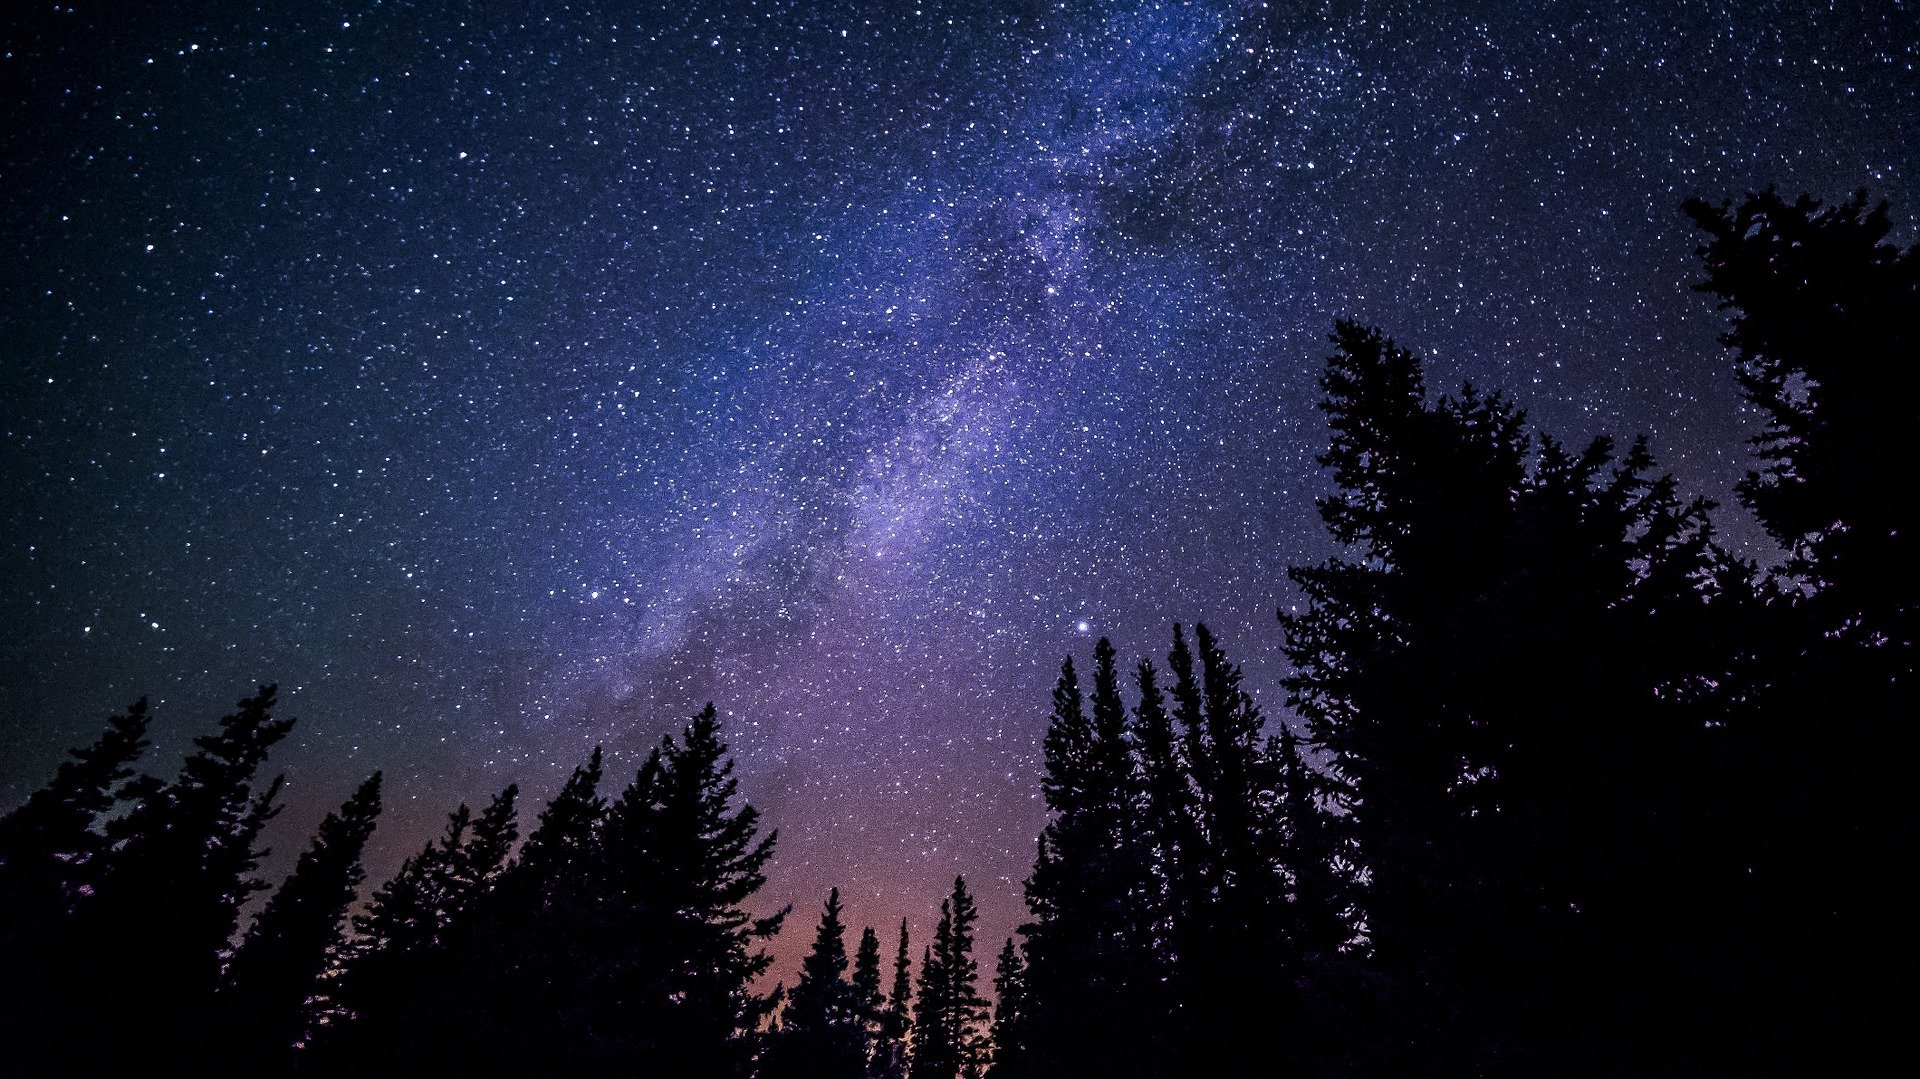
\includegraphics[scale=0.20]{images/milky-way-984050_1920.jpg}
\justify{}
We've reached the point where it's time to assemble all our functional
blocks into a proper lab using resources of a cloud service provider.

\section{Getting Started}

\subsection{Setting up AWS}
\justify{}
Establish an AWS account.

\subsection{Install Docker}
\justify{}
Install Docker on your local machine. Create a Dockerfile and
docker-compose.yml.

\subsection{Configure Project Repository}
\justify{}
Create a GitHub repo for our project. Clone the repo. Copy the
Dockerfile and docker-compose.yml into the new project directory. Create
a branch. Commit the files to the branch and push to repo on GitHub.
Merge the branch, then do a pull to sync your local clone.

\subsection{Configure Testing}
\justify{}
Walk through the steps of adding GitHub Actions that will validate the
Terraform we will be writing to establish our lab infrastructure.

\section{Infrastructure}

\subsection{Lab Diagram}
\justify{}
Let's take a look at the lab environment we intend to create.

\subsection{Add a Makefile}
\justify{}
Add a Makefile that will respond to the ``make docker'' command.

\subsection{Create a Host with Packer}

\subsection{Write Some Terraform Files}

\subsection{Applications}

\subsection{Python Application}

\subsection{Extras}

\subsection{Add a Firewall}
\justify{}
Every keep needs walls around the castle to stop the bad guys from
getting in. The Palo Alto VM-300 series firewall is available as an
image that can be installed in AWS or GCP as desired.
